\begin{figure}[t]
\centering
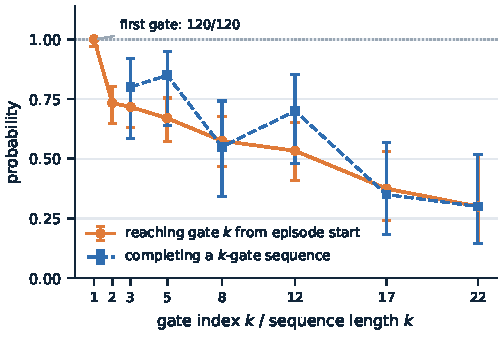
\includegraphics[width=0.72\linewidth]{figures/generated/learning_survival.pdf}
\caption{Multi-gate survival of the frozen learned policy on the pre-registered
validation set, with Wilson $95\%$ intervals. Solid: the unconditional
probability of reaching gate $k$ measured from episode start. Dashed: the
probability of completing an independent $k$-gate sequence. Crossing the first
gate succeeds in $120/120$ episodes, but the full first transition succeeds in
only $88/120$, so more than a quarter of episodes are lost at the first
re-acquisition. Survivor-conditioned transition rates, which average $0.820$ over
all 500 cases, conceal exactly this.}
\label{fig:learning_survival}
\end{figure}
